\chapter{Das erste Kapitel}

In diesem Kapitel soll erklärt werden, wie Text richtig eingefügt werden kann. Außerdem werden Beispiele zur Nutzung von Bildern, Tabellen, Listings, mathematischen Formeln und Listen gezeigt.

Das ist die Vorlage der Technischen Hochschule Ulm



Fangen wir mit dem Text an. Einen neuen Absatz beginnt man damit, dass eine Leerzeile in der tex-Datei gelassen wird. Dabei ist es egal, wie viele Leerzeilen dazwischen sind.
Zeilenumbrüche ohne eine leere Zeile machen jedoch keinen Unterschied und werden wie ein Leerzeichen behandelt. Zur Erklärung der     Leerzeichen:   Zwischen Wörtern wird nie mehr als ein    Leerzeichen    eingebaut.

\textit{Kursiv} schreiben kann man mit \texttt{\textbackslash{}textit\{\}}, \textbf{fett} schreiben mit \texttt{\textbackslash{}textbf\{\}} und \underline{unterstreichen} mit \texttt{\textbackslash{}underline\{\}}. In \enquote{Anführungszeichen} lassen sich Wörter mit dem Befehl \texttt{\textbackslash{}enquote\{\}} setzen. Selbstverständlich lassen sich solche Befehle auch \textit{\textbf{\underline{\enquote{kombinieren}}}}. Außerdem kann mit \texttt{\textbackslash{}texttt\{\}} in \texttt{Code-Schriftart} geschrieben werden, was gerade zur Erklärung von Befehlen oder Listings nützlich sein kann.

\section{Erste Überschrift}
Hiermit sollen Unterkapitel gezeigt werden.

\section{Zweite Überschrift}
Text\cite{Lieb2004}

\subsection{Erste Unter-Überschrift}
Text

\subsection{Zweite Unter-Überschrift}
Text

\subsubsection{Erste Unter-Unter-Überschrift}
Text

\subsubsection{Zweite Unter-Unter-Überschrift}
Text


\section{Abbildungen}
Im Folgenden findet sich eine Beispielabbildung.

\begin{figure}[H]
    \centering
    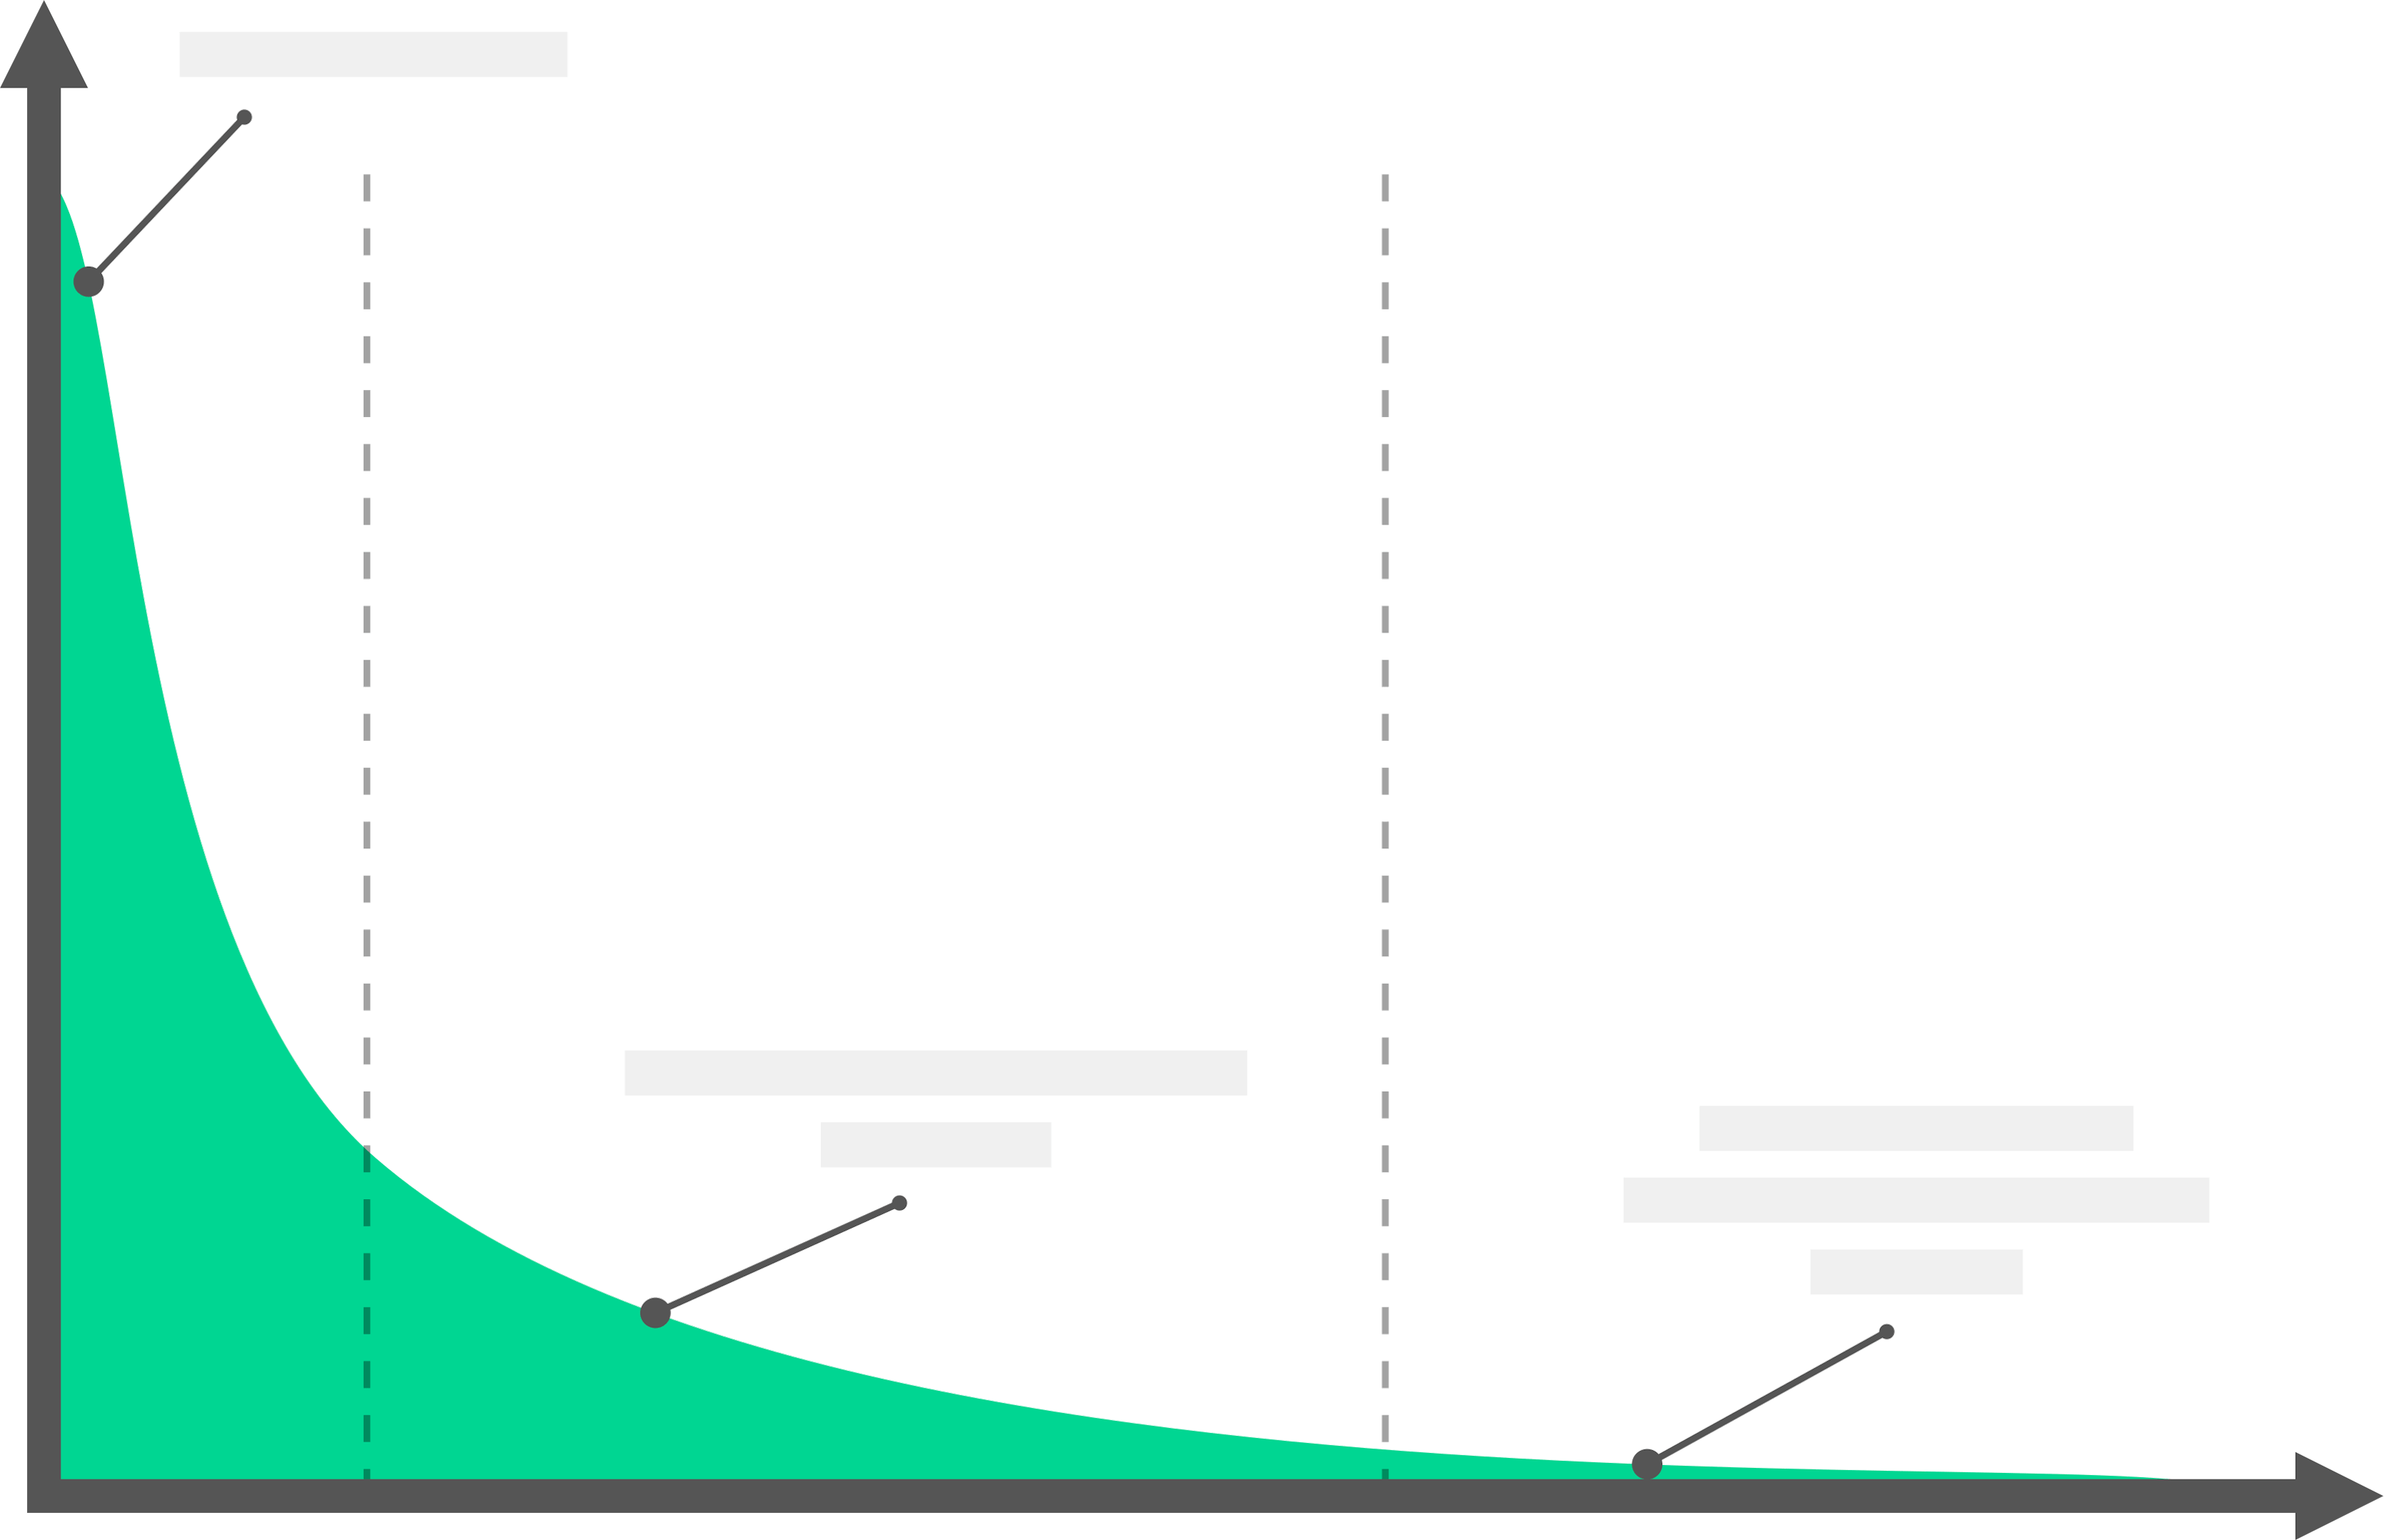
\includegraphics[width=0.7\linewidth]{FigureExample.png}
    \caption{Meine Beispielabbildung}
    \label{fig:beispiel}
\end{figure}

Das aufzurufende Bild sollte hierbei in den Ordner /content/images hochgeladen werden. Die Breite des Bildes lässt sich mit dem \texttt{width}-Parameter einstellen. In diesem Fall nimmt das Bild 70\% der Textbreite ein (also \texttt{width=0.7\textbackslash{}textwidth}). Die 0.7 kann Werte zwischen 0 und 1 annehmen, wobei das Bild beim Wert 1 dann die ganze Textbreite einnimmt.

Es wird empfohlen, genau diesen Code herauszukopieren, um in selber Art und Weise andere Bilder einzufügen. Der Befehl \texttt{\textbackslash{}label\{\}} ist jedoch nur notwendig, wenn man später im Text wieder auf die Abbildung verweisen will.

Das Label darf frei benannt werden, darf jedoch nicht mehr als ein Mal gleich definiert werden. Wie also in Abbildung \ref{fig:beispiel} zu sehen ist, ist das Verweisen auf Bildern ganz einfach. Dazu benötigt man lediglich den \texttt{\textbackslash{}ref\{\}}-Befehl.

\subsubsection{Pro-Tipp:}
Es wird empfohlen, wenn möglich, Vektorgrafiken zu benutzen. Diese brauchen meist weniger Speicherplatz und sind wesentlich besser aufgelöst als andere pixelbasierte Formate. Um SVG nutzen zu wollen, muss der Befehl \texttt{\textbackslash{}includesvg[]\{\}} benutzt werden.

\section{Plots aus CSV-Dateien}
Im Folgenden findet sich ein Beispielplot.

\begin{figure}[H]
    \centering
    \begin{tikzpicture}
        \begin{axis}[
            xlabel={X-Achse},
            ylabel={Y-Achse},
            grid=major,
            width=10cm,
            height=6cm
        ]
            % Daten aus der CSV-Datei laden
            \pgfplotstableread[col sep=comma]{content/images/Example.csv}\datatable
            % Plot der Daten
            \addplot table \datatable;
        \end{axis}
    \end{tikzpicture}
    \caption{Plot aus einer CSV-Datei}
    \label{fig:beispielplot}
\end{figure}

Auch die CSV-Datei sollte in den Ordner /content/images hochgeladen werden. Mit den Parametern \texttt{xlabel} und \texttt{ylabel} können die Beschriftungen der Koordinatenachsen festgelegt werden. 

Mit \texttt{grid} können die Gitterlinien angezeigt oder ausgeblendet werden. Die erlaubten Werte für \texttt{grid} sind folgende: \texttt{none, major, minor, both}. Des Weiteren können der Linienstil und die Linienfarbe angepasst werden für jeweils x-Achse und / oder y-Achse.

Die Größe des Plots kann mit den beiden Parametern \texttt{widh} und \texttt{height} angepasst werden.




\section{Tabellen}

Hier wird das Einfügen einer Tabelle erklärt.

\begin{table}[H]
    \centering
    \caption{Meine Beispieltabelle}
    \label{tab:beispiel}
    \begin{tabular}{|c|c|}
        \hline
        Zelle A1 & Zelle A2 \\
        \hline
        Zelle B1 & Zelle B2 \\
        \hline
    \end{tabular}
\end{table}

Wichtig ist hierbei, dass die Caption gemäß dem Corporate Design immer über der Tabelle stehen muss. Die eigentliche Tabelle (zwischen \texttt{\textbackslash{}begin\{tabular\}} und \texttt{\textbackslash{}end\{tabular\}} ist ein wenig gewöhnungsbedürftig und nicht unbedingt selbsterklärend zu bearbeiten. Aus diesem Grund gibt es verschiedene Tools im Internet, die dir dabei helfen können, eine in LaTeX richtig formatierte Tabelle zu erstellen. Zum Beispiel \href{https://www.tablesgenerator.com/}{https://www.tablesgenerator.com/} oder \href{https://www.latex-tables.com/}{https://www.latex-tables.com/}.

Es wird empfohlen, genau diesen Code herauszukopieren, um in selber Art und Weise andere Tabellen einzufügen. Der Befehl \texttt{\textbackslash{}label\{\}} ist jedoch nur notwendig, wenn man später im Text wieder auf die Tabelle verweisen will.

Das Label darf frei benannt werden, darf jedoch nicht mehr als ein Mal gleich definiert werden. Wie also in Tabelle \ref{tab:beispiel} zu sehen ist, ist das Verweisen auf Tabellen ganz einfach. Dazu benötigt man lediglich den \texttt{\textbackslash{}ref\{\}}-Befehl.


\section{Mathematische Formeln}
Mathematische Formeln werden wie folgt eingefügt.

\begin{equation}
t-t_{0}=\sqrt{\frac{l}{g}}\int_{0}^{\varphi}{\frac{d\psi}{\sqrt{1-k^{2}\sin^{2} {\psi}}}} = \sqrt{\frac{l}{g}} F(k,\varphi)
\label{eq:Beispiel}
\end{equation}
\eqcaption{Beispiel-Titel im Formelverzeichnis}

Der Befehl \texttt{\textbackslash{}label\{\}} ist nur notwendig, wenn man später im Text wieder auf die Formel verweisen will.

Das Label darf frei benannt werden, darf jedoch nicht mehr als ein Mal gleich definiert werden. Wie also in der Formel \ref{eq:Beispiel} zu sehen ist, ist das Verweisen auf Formeln ganz einfach. Dazu benötigt man lediglich den \texttt{\textbackslash{}ref\{\}}-Befehl.

Es gibt verschiedene Tools im Internet, die dabei helfen, eine Formel oder eine Gleichung nach LaTeX umzuwandeln. Hier ein Beispiel: \href{https://latex.codecogs.com/eqneditor/editor.php}{https://latex.codecogs.com/eqneditor/editor.php}


\section{Listings}
Mit Listings kann man essenzielle Teile seines Programm-Codes einbeziehen.

\begin{lstlisting}[caption=Mein Beispiellisting, label=lst:beispiel, language=C++]
public class HelloWorld {
	public static void main (String[] args) {
		// Ausgabe: Hello World!
		System.out.println("Hello World!");
	}
}
\end{lstlisting}

Das Listing formatiert den Code direkt sprachspezifisch in den richtigen Farben. Leerzeichen in Strings werden ebenfalls hervorgehoben. Dafür muss nur der Parameter \texttt{language=...} angepasst werden.

Es wird empfohlen, genau diesen Code herauszukopieren, um in selber Art und Weise andere Tabellen einzufügen. Der Befehl \texttt{label=...} ist jedoch nur notwendig, wenn man später im Text wieder auf das Listing verweisen will.

Das Label darf frei benannt werden, darf jedoch nicht mehr als ein Mal gleich definiert werden. Wie also in Listing \ref{lst:beispiel} zu sehen ist, ist das Verweisen auf Listings ganz einfach. Dazu benötigt man lediglich den \texttt{\textbackslash{}ref\{\}}-Befehl.


\section{Listen}
Manchmal braucht man auch eine Liste, um Aufzählungen aufzuführen. Diese erstellt man wie folgt.

\begin{itemize}
\item Der erste Punkt.
\item Der zweite Punkt.
\item Der dritte Punkt.
\end{itemize}

Das geht auch mit Zahlen:

\begin{enumerate}
\item Der erste Punkt.
\item Der zweite Punkt.
\item Der dritte Punkt.
\end{enumerate}

\section{Schaltpläne}
Möchte man Schaltpläne mit LaTeX zeichnen, so ist dies möglich. Für komplexere Schaltpläne muss man sich in die Dokumentation des packages \texttt{circuitikz} einlesen. Ein kleines Beispiel ist im Folgenden gegeben:

\begin{circuitikz} \draw
  (0,0) to[battery1, l=$V_{in}$] (0,4)
  to[resistor, l=$R_1$] (4,4)
  to[resistor, l=$R_2$] (4,0)
  -- (0,0);
\end{circuitikz}